\documentclass[]{elsarticle} %review=doublespace preprint=single 5p=2 column
%%% Begin My package additions %%%%%%%%%%%%%%%%%%%
\usepackage[hyphens]{url}
\usepackage{lineno} % add
\bibliographystyle{elsarticle-harv}
\biboptions{sort&compress} % For natbib
\usepackage{graphicx}
\usepackage{booktabs} % book-quality tables
%% Redefines the elsarticle footer
%\makeatletter
%\def\ps@pprintTitle{%
% \let\@oddhead\@empty
% \let\@evenhead\@empty
% \def\@oddfoot{\it \hfill\today}%
% \let\@evenfoot\@oddfoot}
%\makeatother

% A modified page layout
\textwidth 6.75in
\oddsidemargin -0.15in
\evensidemargin -0.15in
\textheight 9in
\topmargin -0.5in
%%%%%%%%%%%%%%%% end my additions to header

\usepackage[T1]{fontenc}
\usepackage{lmodern}
\usepackage{amssymb,amsmath}
\usepackage{ifxetex,ifluatex}
\usepackage{fixltx2e} % provides \textsubscript
% use upquote if available, for straight quotes in verbatim environments
\IfFileExists{upquote.sty}{\usepackage{upquote}}{}
\ifnum 0\ifxetex 1\fi\ifluatex 1\fi=0 % if pdftex
  \usepackage[utf8]{inputenc}
\else % if luatex or xelatex
  \usepackage{fontspec}
  \ifxetex
    \usepackage{xltxtra,xunicode}
  \fi
  \defaultfontfeatures{Mapping=tex-text,Scale=MatchLowercase}
  \newcommand{\euro}{€}
\fi
% use microtype if available
\IfFileExists{microtype.sty}{\usepackage{microtype}}{}
\usepackage{graphicx}
% We will generate all images so they have a width \maxwidth. This means
% that they will get their normal width if they fit onto the page, but
% are scaled down if they would overflow the margins.
\makeatletter
\def\maxwidth{\ifdim\Gin@nat@width>\linewidth\linewidth
\else\Gin@nat@width\fi}
\makeatother
\let\Oldincludegraphics\includegraphics
\renewcommand{\includegraphics}[1]{\Oldincludegraphics[width=\maxwidth]{#1}}
\ifxetex
  \usepackage[setpagesize=false, % page size defined by xetex
              unicode=false, % unicode breaks when used with xetex
              xetex]{hyperref}
\else
  \usepackage[unicode=true]{hyperref}
\fi
\hypersetup{breaklinks=true,
            bookmarks=true,
            pdfauthor={},
            pdftitle={Short Paper},
            colorlinks=true,
            urlcolor=blue,
            linkcolor=magenta,
            pdfborder={0 0 0}}
\urlstyle{same}  % don't use monospace font for urls
\setlength{\parindent}{0pt}
\setlength{\parskip}{6pt plus 2pt minus 1pt}
\setlength{\emergencystretch}{3em}  % prevent overfull lines
\setcounter{secnumdepth}{0}
% Pandoc toggle for numbering sections (defaults to be off)
\setcounter{secnumdepth}{0}
% Pandoc header


\usepackage[nomarkers]{endfloat}

\begin{document}
\begin{frontmatter}

  \title{Short Paper}
    \author[Some Institute of Technology]{Alice Anonymous}
   \ead{alice@example.com} 
  
    \author[Another University]{Bob Security}
   \ead{bob@example.com} 
  
    
  \begin{abstract}
  This is the abstract.
  
  It consists of two paragraphs.
  \end{abstract}
  
 \end{frontmatter}

\begin{center}
\Large\scshape{Explosive Prices for South African Art} \\ 
\vspace{1em}
\large\normalfont{Laurie Binge}\footnote{PhD candidate at the Department of Economics at Stellenbosch University.} \\
\large\normalfont{Willem H. Boshoff}\footnote{Associate Professor at the Department of Economics at Stellenbosch University.} \\
\normalsize\textit{Stellenbosch University} \\
\normalsize\normalfont{\today} 
\end{center}\begin{small}

South African art has experienced a surge in popularity over the last few decades, with large price increases and record prices at local and international auctions. This paper looks for evidence of a bubble in the South African art market by testing for mildly explosive prices. The outcome of the test depends critically on the estimation of a reasonably accurate quality-adjusted price index, which can be challenging for unique assets such as art. The choice of methodology determines whether there is compelling evidence of a bubble and what origination and termination dates are identified. This paper estimates three sets of art price indices, based on the three main methodologies used to estimate quality-adjusted price indices for unique assets. The regression-based indices seem to point to consistent evidence of explosive price behaviour in the run-up to the financial crisis. Further analysis indicates that the bubble was relatively dispersed throughout the market, although prices seem to have been especially explosive for high-end oil paintings by the top artists. 

\vspace{0.5em}
\noindent{\textbf{JEL Classification:} C43, Z11, E31, G12} \\
\noindent{\textbf{Keywords:} South African Art, Hedonic Price Index, Pseudo Repeat Sales, Explosive Prices }
\end{small}\renewcommand{\thefootnote}{\arabic{footnote}}

\section{Introduction}\label{introduction}

South African art has experienced a surge in popularity over the last
few decades. The South African art market is relatively established and
well-developed, and has grown markedly over the last two decades, both
in terms of the number of transactions and total turnover (Fedderke and
Li 2014). Artworks by South African artists have exhibited large price
increases and have reached record prices at international and local
auctions, both for the country's ``masters'' - including Irma Stern,
Walter Battiss, and JH Pierneef - and contemporary artists like William
Kentridge (Naidoo 2013). In 2011, for instance, Bonhams in London sold
Irma Stern's \emph{``Arab Priest''} for a hammer prices of £2.7 million,
a world record for a South African artwork at auction. Also in 2011,
Stern's \emph{``Two Arabs''} was sold by Strauss \& Co. for a hammer
price of R19 million, a record for a South African auction.

The increase in the popularity of South African art, both locally and
abroad, has sparked a vibrant market for collectors and investors. The
interest in South African art, at least partly as an investment vehicle,
is commensurate with international trends, where fine art has become an
important alternative asset class in its own right (Renneboog and
Spaenjers 2015). In addition to the potential for appreciation in value,
artworks may be used to aid portfolio diversification, as collateral for
loans, or to take advantage of slacker regulatory and tax rules. Thus,
unlike pure financial investments, artworks are durable goods with
consumption and investment good characteristics (Renneboog and Spaenjers
2015).

The large price increases and record prices for South African artworks
at local and international auctions, especially between 2008 and 2011,
prompted commentators at the time to claim that the market was
overheating and suggest the possibility of a ``bubble'' in the market
(e.g. Rabe (2011); Hundt (2010); Curnow (2010)). According to the New
Palgrave Dictionary of Economics, ``\emph{bubbles refer to asset prices
that exceed an asset's fundamental value because current owners believe
they can resell the asset at an even higher price}'' (Brunnermeier
2008). A bubble consists of a sharp rise in a given asset price, above a
level sustainable by fundamentals, followed by a sudden collapse
(Kräussl, Lehnert, and Martelin 2016).

When it comes to the art market, however, it is particularly challenging
to determine the fundamental value from which prices potentially
deviate. In the case of stocks, dividends have been used to obtain the
expected cash flow as a measure of fundamental value. Rents and
convenience yields can potentially be used for real estate prices and
commodity prices (Penasse and Renneboog 2014). In contrast, artworks do
not generate a future income stream (e.g.~dividends or rents) that can
be discounted to determine the fundamental value. Artworks usually have
little inherent value, unless the materials used have a high intrinsic
value (Spaenjers, Goetzmann, and Mamonova 2015). Instead, artworks are
acquired for a kind of non-monetary utility or aesthetic dividend,
sometimes described as ``aesthetic pleasure'' (Gérard-Varet 1995). This
dividend can be seen as the rent one would be willing to pay to own the
artwork over a given period. It can reflect aesthetic pleasure, but may
also provide additional utility as the signal of wealth (Mandel 2009).
The price of an artwork should equal the present value of future private
utility dividends over the holding period, plus the expected resale
value. The value of the dividend is unobservable and is likely to vary
greatly across collectors, based on their motivations and
characteristics (Penasse and Renneboog 2014). Thus, it almost impossible
to determine the fundamental value of art (Kräussl, Lehnert, and
Martelin 2016).

To overcome this issue, this paper follows Kräussl, Lehnert, and
Martelin (2016) in using a direct method of bubble detection developed
by Peter C B Phillips, Wu, and Yu (2011). The approach is based on a
right-tailed augmented Dickey-Fuller (ADF) test, which can detect
explosive behaviour directly in time series. Peter C B Phillips, Wu, and
Yu (2011) originally applied the method to stock prices. They showed
that there was evidence of explosiveness in stock prices, but not
dividend yields, implying that price explosiveness could not be
explained by developments in fundamentals.

The test, however, requires the estimation of a reasonably accurate
quality-adjusted price index, which can be challenging for unique assets
such as art and real estate. The choice of methodology will determine
whether there is compelling evidence of a bubble and what origination
and termination dates are identified. Each methodology has shortcomings
and the danger is that the biases inherent in each methodology may be
driving the results.

This paper uses three broad methodologies to develop quarterly price
indices for South African art. The use of quarterly indices allows the
paper to investigate higher frequency movements in art prices. Simple
central tendency indices are estimated as a baseline for comparison, but
do not adequately control for quality-mix changes over time. The hedonic
regression method is able to control more adequately for quality-mix
changes, but has the shortcoming of potential omitted variable bias.
Repeat sales indices suffer less from potential omitted variable bias,
but have the shortcoming of potential sample selection bias. In this
case the scarcity of repeat sales observations in the database limits
the usefulness of the classical repeated sales approach. The paper
proposes a simple hybrid repeat sales method to address the problem of
scarcity of repeat sales observations and to some extent the potential
omitted variable bias inherent in the hedonic method. The paper then
compares and evaluates the indices in terms of smoothness, which helps
to determine the bubble period more accurately.

The regression-based indices seem to point to consistent evidence of
mildly explosive price behaviour in the run-up to the financial crisis,
between 2005/06 and 2008. Different segments of the market are then
investigated to find out whether this bubble was dispersed throughout
the market. The results indicate that the bubble was relatively
dispersed, although prices seem to have been especially explosive for
high-end oil paintings by the top artists.

\section{South African Art Auction
Data}\label{south-african-art-auction-data}

The literature on estimating art price indices has relied almost
exclusively on publicly available auction prices. It is generally
accepted that auction prices set a benchmark that is also used in the
private market (Candela and Scorcu 2001; Renneboog and Spaenjers 2013).
Private sales prices are likely anchored by auction prices and are
likely to be highly correlated over time for similar artworks, even if
their levels are different (Olckers, Kannemeyer, and Stevenson 2015).
This paper relies on publicly available auction prices, which are the
only consistently available price data for the South African art market.

The indices are based on data recorded by AuctionVault. This data cover
sales of South African art at 8 auction houses\footnote{These are: 5th
  Avenue, Ashbeys, Bernardi, Bonhams, Christies, Russell Kaplan, Stephan
  Welz \& Co and Strauss \& Co.} between 2000 and 2015. The database
includes 52,059 sales by 4,123 different artists. The following
characteristics are available for each auction record: hammer price,
artist name, title of work, medium, size, whether or not the artwork is
signed, dated and titled, auction house, date of auction, and the number
of distinct works in the lot.

Strauss \& Co and Stephan Welz \& Co are the two local auction houses
that have handled the bulk of sales in recent years, with auctions in
Cape Town and Johannesburg. Bonhams in London is the only major
international auction house with a dedicated South African art
department, and has two major South African art sales annually. The
auction houses follow an open ascending auction, where the winner pays
the highest bid. A sale is only made if the hammer price is above the
secret reserve price. Otherwise the artwork is unsold and is said to be
bought in (Fedderke and Li 2014). Like most studies, the database lacks
information on buy-ins and the analysis is forced to disregard the
potential sample selection problem. The following section briefly
discusses the variables available in the database and included in models
of art prices.

\subsection{Artwork characteristics}\label{artwork-characteristics}

\emph{Artist reputation}: Hedonic models typically include dummy
variables to control for the artists. However, some artists often have
to be excluded from estimation, due to a lack of degrees of freedom.
Alternatively, a reputation variable can be constructed, either from the
art literature, or from the auction data itself. The models in this
paper are estimated using a continuous reputation variable estimated
with the 2-step hedonic approach suggested by Kräussl and Van Elsland
(2008). This approach allows the use of every auction record, instead of
only those auction records that belong to a sub-sample of selected
artists.

\emph{Size}: The most common variable used to describe the physical
characteristics of an artwork is its size or surface area. The models
use the natural logarithm of the surface area of the artwork in
\(cm^2\). The models also include size and medium interaction terms.
This is particularly important for sculptures, as the size of a
sculpture is usually only recorded in terms of its height (in cm).

\emph{Auction house}: Dummy variables for the auction houses are also
typically included. The more prominent auction houses usually have a
positive effect on prices. One reason might be that the more renowned
auction houses will offer higher quality work (Kräussl and Logher 2010).
Thus, the variables might be picking up otherwise unobservable quality
differences and do not necessarily reflect auction house certification
(Renneboog and Spaenjers 2013). Moreover, different auction houses
charge different commissions to both buyers and sellers. For example,
Strauss \& Co reported a buyer's premium of 10\%-15\%, while Bonhams
charged premiums of up to 25\% (Olckers, Kannemeyer, and Stevenson
2015). The hammer prices exclude these premiums and are therefore not a
perfect measure of the cost to the buyer and revenue to the seller. For
the purposes of a price index the auction house dummies should capture
the different premiums charged by the auction houses.

\emph{Mediums}: Average prices vary across mediums. This might be due to
the durability of the medium, the stage of production the medium is
associated with (e.g.~preparatory drawings) and in some cases the
replacement value of the materials used (e.g.~sculptures cast in
bronze). Oil paintings traditionally earn the highest prices. The
availability of copies may decrease the prices of prints and photographs
relative to other mediums. Studies typically include dummy variables for
the different mediums as defined in their data (Kräussl and Logher
2010). The models use the 9 mediums defined in the dataset; the same
mediums used by Olckers, Kannemeyer, and Stevenson (2015).

\emph{Authenticity dummies}: Models often include dummies for whether
the artwork is signed and dated. There might be a premium for these
attributes, as there is less uncertainty about authenticity (Renneboog
and Spaenjers 2015). These dummies are included in the models and are
expected to have positive coefficients.

\emph{Number of works in the lot}: The models also control for cases in
which more than one artwork was sold in the same auction lot. This is
because the recorded size corresponded to each artwork separately and
not the group. Moreover, it is possible that lots including more than
one artwork fetch a lower price per artwork than if they sold
separately.

\section{Methodology}\label{methodology}

\subsection{Estimating Art Price
Indices}\label{estimating-art-price-indices}

The construction of price indices for unique assets is challenging for
at least two reasons (Jiang, Phillips, and Yu 2014). Firstly, the low
frequency of trading means that only a subset of the market is traded at
a given time, while the prices of non-transacted items are unobservable.
Secondly, the heterogeneity of these items means that the quality of
assets sold is not constant over time. Thus, the composition of items
sold will generally differ between periods, making it difficult to
compare prices over time (Hansen 2009). Constructing an index for unique
assets, such as artworks, therefore requires a different approach than
is used for indices of stocks, bonds and commodities. Four broad
measurement techniques have been used to construct these indices:
central tendency, hedonic, repeat sales, and hybrid methods (Eurostat
2013).

\subsubsection{Central Tendency Methods}\label{central-tendency-methods}

The simplest way to construct a price index is to calculate a measure of
central tendency from the distribution of prices. The median is often
preferred to the mean as a measure of central tendency, because price
distributions are generally positively skewed (Hansen 2009). These
average measures have the advantage of being simple to construct and do
not require detailed data. Despite its advantages, an index based on
average prices does not account for the difficulties mentioned above.
For assets such as artworks, central tendency indices may be more
dependent on the mix of objects that come to market than changes in the
underlying market. If there is a correlation between turning points in
asset price cycles and compositional and quality changes, then an
average could be especially inaccurate (Hansen 2009).

Stratified central tendency measures can control for compositional
changes in assets sold over time to some extent, by separating the
sample into subgroups according to individual characteristics such as
artist and medium. After constructing a measure of the central tendency
for each subgroup, the aggregate mix-adjusted index is typically
calculated as a weighted average of the indices for the subgroups
(e.g.~a Fisher index) (Eurostat 2013). However, these mix-adjusted
measures adjust only for the variation in the quality of assets across
the subgroups. The number of subgroups may be increased to reduce the
quality-mix problem, if the data permits, although some quality-mix
changes will likely remain (Hansen 2009). However, this will reduce the
average number of observations per subgroup and raise the standard error
of the overall index (Eurostat 2013). If the subgroups become very
small, small changes can have a large impact on the index. As a
consequence of these difficulties, the repeat sales and hedonic methods
have dominated the international literature, especially with regard to
art price indices.

Two central tendency price indices are estimated at a quarterly
frequency to act as a baseline in comparing the indices resulting from
the different methodologies. The median index is simply the median price
for each quarter. The Fisher index is a mix-adjusted central tendency
index, which is stratified by artist and medium. The base periods are
allowed to vary for each index point and the index points are then
chained together to form the overall chain-link index.

\subsubsection{Hedonic Methods}\label{hedonic-methods}

The hedonic method is derived from the microeconomic theory of implicit
prices, which supposes that utility is derived from the characteristics
or attributes of goods (Lancaster 1966). Griliches (1961) first applied
the hedonic method for the valuation of automobiles. Rosen (1974)
provides a theoretical framework in which the hedonic price function
emerges from the interaction between buyers and sellers.

The hedonic method controls for quality-mix changes by attributing
implicit prices to a set of value-adding characteristics of the
individual item. Hedonic regressions control for the observable
attributes of an asset to obtain an index reflecting the price of a
``standard asset'' (Renneboog and Van Houtte 2002). The approach entails
regressing the logarithm of the sales price on the relevant attributes.
The standard hedonic model usually takes the following form:
\[\ln P_{it} = \sum_{t=1}^T \delta_t D_{it} + \sum_{j=1}^J \beta_{jt} X_{jit} + \sum_{k=1}^K \gamma_{kt} Z_{kit} + \epsilon_{it}\]
where \(P_{it}\) represents the price of item \(i\) at time \(t\)
\((t=1, ..., T)\); \(D_{it}\) is a time dummy variable taking the value
of 1 if item \(i\) is sold in period \(t\) and 0 otherwise, \(X_{jit}\)
is a set of \(j\) \((j=1, ..., J)\) observed attributes of item \(i\) at
time \(t\); \(Z_{kit}\) is a set of \(k\) \((k=1, ..., K)\) unobserved
attributes that also influence the price; and \(\epsilon_{it}\) is a
random (white noise) error term.

The coefficients on the time dummies provide an estimate of the average
increase in prices between periods, holding the change in any of the
measured quality dimensions constant (Griliches 1961). In other words,
they capture the ``pure price effect'' (Kräussl and Lee 2010). The price
index is then simply the series of estimated coefficients:
\(\hat{\delta_1}, ..., \hat{\delta_T}\).

The most common form of the hedonic equation assumes that the implicit
prices (i.e.~the coefficients \(\beta_t\) and \(\gamma_t\)) are constant
over the entire sample. However, when demand and supply conditions
(e.g.~tastes) change, the implicit prices of the attributes may change
(Renneboog and Spaenjers 2013). One way to allow for shifts in
parameters is to employ an adjacent-periods regression (Triplett 2004).
Separate regressions are estimated for adjacent time periods and the
sequence of shorter indices are then chain-linked together to form the
continuous overall index (D. P. McMillen 2012). This method allows the
coefficients, and therefore the implicit prices assigned to the
characteristics, to vary in each regression (Triplett 2004). There is a
trade-off in selecting the length of the estimation window. Shorter
estimation windows decrease the likelihood of large breaks but also
decrease the number of observations used to estimate the parameters
(Dorsey et al. 2010).

In addition to the standard full sample hedonic index, two
adjacent-period indices are calculated by estimating separate models for
1-year and 2-year adjacent sub-samples. A 5-year overlapping-periods
index is also estimated, allowing gradual shifts in the implicit prices
(Shimizu, Nishimura, and Watanabe 2010).

The majority of studies on art price indices have used hedonic models to
construct the indices, due to the lack of repeat sales of artworks and
the availability of information on many of their important attributes.
Anderson (1974) was the first to apply a hedonic regression to art
prices. More recent examples include: Renneboog and Van Houtte (2002),
who estimated an index of Belgian paintings; Kräussl and Lee (2010), who
studied the prices of the top 500 artists in the world; Kräussl and
Logher (2010), who analysed the performance of art in Russia, China and
India; and Kräussl (2015) who analysed art from the Middle East and
Northern Africa region.

The primary difficulty with hedonic price indices is this potential
omitted variable bias. If the functional form is misspecified or omitted
variables are correlated with sales timing, it will result in
misspecification or omitted variable bias, which will bias the indices
(Jiang, Phillips, and Yu 2014). Although omitted variables are a problem
in every model, relatively detailed data is available for art, which
should capture a large part of the variation in sales prices. Omitted
variable bias should therefore be less of a problem than for other
unique assets like real estate, and the omitted variable bias is often
small in practice (Triplett 2004; Renneboog and Spaenjers 2013).

\subsubsection{Repeat Sales Model}\label{repeat-sales-model}

The repeat sales method is an alternative estimation method for
quality-adjusted price indices, based on price changes of items sold
more than once. It was initially proposed by Bailey, Muth, and Nourse
(1963) to calculate house price changes. It was subsequently extended by
Case and Shiller (1987) and is currently used to produce the
S\&P/Case-Shiller Home Price Indices in the US. The repeat sales method
tracks the sale of the same item over time. It aggregates sales pairs
and estimates the average return on the set of items in each period
(Kräussl and Lee 2010). As a result, it does not require the measurement
of quality, only that the quality of each item be constant over time
(Case and Shiller 1987).

The repeat sales model can be derived from the hedonic model, if the
hedonic model is differenced with respect to consecutive sales of items
that have sold more than once in the sample period (D. P. McMillen
2012). In the standard repeat sales model the dependent variable is
regressed on a set of dummy variables corresponding to time periods.
This estimating equation provides unbiased estimates of pure time
effects without having to correctly specify the item attributes or the
functional form of the hedonic equation (Deng, McMillen, and Sing 2012).
By differencing the hedonic equation it also potentially controls for
omitted variables. It also has the advantage of not being data
intensive, as the only information required to estimate the index is the
price, the sales date and a unique identifier (e.g.~the address of the
property).

A few studies have utilised the repeat sales method to estimate art
price indices. These studies have typically relied on very large sales
databases, due to the infrequency of repeat sales of individual
artworks. Mei and Moses (2002) constructed the seminal repeat sales
index of art prices for the period 1875-2000. Their methodology is
currently used to produce the Mei Moses Art Index for Beautiful Asset
Advisors. Other examples include Korteweg (2013) and W. Goetzmann,
Renneboog, and Spaenjers (2011), who used a database of over a million
sales dating back to the 18th century.

A disadvantage of the repeat sales method is the possibility of sample
selection bias. Items that have traded more than once may not be
representative of the entire population of items. For example, if
cheaper artworks sell more frequently than expensive artworks, but
high-quality artworks appreciate faster, a repeat sales index will tend
to have a downward bias (Eurostat 2013). The biggest problem with the
repeat sales method in the current context is that single-sale data is
discarded. This is problematic because the resale of a specific artwork
may only occur infrequently, which substantially reduces the total
number of observations available. Only 515 true repeat sales pairs could
be identified in the sample, which limits the usefulness of the
classical repeated sales approach in this case.

\subsubsection{Hybrid Models}\label{hybrid-models}

An interesting perspective is to view the repeat sales specification as
an extreme solution to a matching problem. The repeat sales approach
requires an exact match to estimate the index. The idea behind the
imperfect matching method proposed by D. P. McMillen (2012) is that some
items may be similar enough to control for many of the differences in
(observable and unobservable) attributes. The objective is to match
sales observations over time, according to some criterion, so as to
cancel out as many as possible of the differences in attributes. This
involves a trade-off between the within-pair ``similarity'' and the
sample size (Guo et al. 2014).

This paper applies a simple hybrid repeat sales model to art prices for
the first time. This procedure is similar in spirit to the ``pseudo
repeat sales'' (ps-RS) procedure suggested by Guo et al. (2014). The
first ps-RS sample is created by matching artworks all the hedonic
attributes, except the title of the artwork. Matching by this criteria
increases the number of repeat sales pairs to 6,642, which includes the
515 true repeat sales or exact matches. The second ps-RS sample allows
the sample to increase further by matching on all the hedonic attributes
except the title and the presence of a signature and date on the
artwork, i.e.~the authenticity dummies. This increases the pseudo repeat
sales sample to 7,965 sales pairs.

The differential hedonic equation is then applied to the pseudo repeat
sales samples, where artwork \(i\) in quarter \(t\) and artwork \(h\) in
quarter \(s\) form a matched pair \((t>s)\):
\[\ln P_{it} - \ln P_{hs} = \sum_{j=1}^J \beta_j (X_{itj} - X_{hsj}) + \sum_{t=0}^T \delta_t G_{it} + \epsilon_{iths}\]
where \(G_{it}\) is again a time dummy equal to 1 if the later sale
occurred in quarter \(t\), -1 if the former sale in the pair occurred in
quarter \(s\), and 0 otherwise; and \(\epsilon_{iths}\) again represents
a white noise residual.

For the first ps-RS sample, the only remaining independent variable is
the difference in the auction house dummies \((X_{it1} - X_{hs1})\).
This takes account of possible differences in quality and commission
structures. In the second ps-RS sample the independent variables
represent the differences in the auction house dummies and the
differences in the two authenticity dummies. The independent variables
therefore include indicators of the relatively small and easy to measure
within-pair differentials in attributes between the two items.

The ps-RS approach mitigates the problem of potential omitted variable
bias with the hedonic method. Taking first differences between similar
items will control for omitted variables when they are the same for the
two items that form the pseudo sales pairs. For example, if Van Gogh's
\emph{Sunflowers} paintings are treated as repeat sales, taking first
differences would control for attributes such as theme, style, material,
prominence, and the stage of the artist's career. Other potentially
significant variables might include an array of interaction and
non-linear terms. The ps-RS approach also mitigates the problems of
small sample sizes and sample selection bias with repeat sales methods
by using more of the transaction data (D. P. McMillen 2012). Calomiris
and Pritchett (2016) used a similar procedure, based on the differential
hedonic equation, in analysing slave price indices. They argued that the
similarities between the indices provided confidence that temporal
variation in unobservable characteristics were not dictating the
results.

There is no consensus regarding the preferred approach of constructing
quality-adjusted price indices, either theoretically or empirically. The
specific methodology adopted is dependent on the data available. Indices
estimated with the different methodologies may provide different results
for the bubble detection tests. The danger is that the biases inherent
in each methodology may be driving the results (e.g.~the omitted
variable bias may be correlated with the cycle).

\subsection{Bubble Detection
Framework}\label{bubble-detection-framework}

The adverse effects of bubbles and their related crises have led to a
large literature on financial crises and the detection of bubbles in
asset prices, including the seminal work by Kindleberger and Aliber
(2005) and the modelling approach by Peter C B Phillips, Wu, and Yu
(2011).

The most commonly used detection methods are based on the present value
model and the rational bubble assumption. According to the present value
model, under rational expectations, the price of an asset is equal to
the present value of its future income stream, i.e.~the expected
fundamental value: \[P_t = \frac{1}{1+r_f} E_t(P_{t+1} + \gamma_{t+1})\]
where \(r_f\) is the constant discount rate, \(P_t\) is the asset price
at time \(t\), and \(\gamma_{t+1}\) is the payment received
(e.g.~dividends, rents or a convenience yield) for owning the asset
between \(t\) and \(t+1\). When \(t+n\) is far into the future,
\(\frac{1}{1+r_f} E_t(P_{t+n})\) does not affect \(P_t\), as it tends to
zero as \(n\) becomes infinitely large. The present value or market
fundamental solution could be written as:
\[F_t = E_t[\sum_{i=1}^n \frac{1}{1+r_f} (\gamma_{t+n})]\]

If a gap between the market fundamental solution and the actual price
exists and the terminal condition does not hold, an additional ``bubble
component'', \(B_t\), has to be added to the solution of equation:
\(P_t = F_t + B_t\) (Yiu, Yu, and Jin 2013). In this case \(F_t\) is
called the fundamental component of the price and \(B_t\) is any random
variable that satisfies the following condition:
\[B_t = \frac{1}{1+r_f} E_t(B_{t+n})\]

The statistical properties of \(P_t\) are determined by those of \(F_t\)
and \(B_t\). In the absence of a bubble, when \(B_t=0\), the degree of
non-stationarity in \(P_t\) is controlled by the nature of the series
\(F_t\), which in turn is determined by the properties of \(\gamma_t\).
The current price of the commodity is therefore determined by market
fundamentals: for example, if \(\gamma_t\) is an I(1) process then
\(P_t\) would be an I(1) process.

When a bubble is present, if \(B_t \neq 0\), current prices \(P_t\) will
exhibit explosive behaviour, as \(B_t\) reflects a stochastic process in
which the expected value of next period's value, forecast on the basis
of the current period's information, is greater than or equal to the
current period's value (Kräussl, Lehnert, and Martelin 2016). In the
absence a structural change in the fundamental process or explosiveness
in the fundamentals, a period of explosive prices must have a
non-fundamental explanation. Under the assumed properties of
\(\gamma_t\), the observation of mildly explosive behaviour in \(P_t\)
(i.e.~non-stationarity of an order greater than unit root
non-stationarity) will offer evidence of bubble behaviour. This
expression embodies an explosive property and introduces ``bubble''
movements in the price over the fundamental component (Areal, Balcombe,
and Rapsomanikis 2013). Thus, the theory predicts that if a bubble
exists, prices should inherit its explosiveness property. This enables
the formulation of statistical tests that try to detect evidence of
explosiveness in the data (Caspi 2013).

Given the different stochastic properties of the fundamental and bubble
components, early tests were based on unit root and cointegration tests.
Campbell and Shiller (1987) suggested a unit root test for explosiveness
in prices, based on the idea that the gap between the asset price and
the fundamental value will exhibit explosive behaviour during the
process of bubble formation. Diba and Grossman (1988) showed that if
fundamental values are not explosive, the explosive behaviour in prices
is a sufficient condition for the presence of bubble.

However, unit root and cointegration tests are not capable of detecting
explosive prices when a series contains periodically collapsing bubbles.
Evans (1991) showed that these tests could not differentiate between a
periodically collapsing bubble and a stationary process. A series
containing periodically collapsing bubbles could therefore be
interpreted by the standard unit root tests as a stationary series,
leading to the incorrect conclusion that the data contained no explosive
behaviour (Peter C B Phillips, Wu, and Yu 2011).

A number of methods have been proposed to deal with this critique (Yiu,
Yu, and Jin 2013). The recursive tests proposed by Peter C B Phillips,
Wu, and Yu (2011) and Peter Charles Bonant Phillips, Shi, and Yu (2012)
are not subject to this criticism and can effectively distinguish unit
root processes from periodically collapsing bubbles, as well as
date-stamp their origin and collapse. The tests proposed by Peter C B
Phillips, Wu, and Yu (2011) are based on the idea of repeatedly
implementing a right-tailed unit root test. The method involves the
estimation of an autoregressive model, starting with a minimum fraction
of the sample and incrementally expanding the sample forward.

The model typically takes the following form:
\[\Delta y_t = \alpha_w + (\delta_w - 1) y_{t-1} + \sum_{i=1}^k \phi_w^i \Delta y_{t-i} + \epsilon_t\]
where \(y_t\) is the asset price series, \(\alpha\), \(\delta\) and
\(\phi\) are the parameters to be estimated, \(w\) is the sample window
size, \(k\) is the lag order, and \(\epsilon_t\) is the white noise
error term.

A sample of Augmented Dickey-Fuller test statistics are calculated from
each regression. The null hypothesis of a unit root \((\delta = 1)\) is
tested against the right-tailed alternative of mildly explosive
behaviour \((\delta > 1)\). The supremum value of the ADF sequence is
then used to test for mildly explosive behaviour. By looking directly
for evidence of explosive behaviour, the test avoids the risk of
misinterpreting a rejection of the null hypothesis due to stationary
behaviour.

The method also allows for date-stamping of the origination and
termination dates by matching the time series of the recursive test
statistics to the critical value sequence. In other words, each element
of the estimated ADF sequence is compared to the corresponding
right-tailed critical values of the ADF statistic to identify a bubble
period. The estimated origination point of a bubble is the first
observation in which ADF value crosses the corresponding critical value
(from below), while the estimated termination point is the first
observation thereafter when the ADF value crosses below the critical
value (Caspi 2013). Simulations by Homm and Breitung (2012) indicated
that the procedure worked satisfactorily against other time series tests
for the detection of bubbles and was particularly effective for
real-time bubble detection.

Various studies have used the method to investigate bubbles in a number
of asset markets, including real estate (Jiang, Phillips, and Yu 2014;
Balcilar, Katzke, and Gupta 2015), commodities (Areal, Balcombe, and
Rapsomanikis 2013; Figuerola-Ferretti, Gilbert, and Mccrorie 2015) and
art (Kräussl, Lehnert, and Martelin 2016). The results from these
studies have often suggested the existence of periods of explosive
prices between 2006/07 and 2008.

\section{Results}\label{results}

\subsection{Art Price Indices}\label{art-price-indices}

Figure 1 illustrates representative indices for the three methodologies:
median index, the 1-year adjacent period hedonic index and the second
version (larger sample) of the ps-RS index. The two regression-based
indices seem to point to a similar general trend in South African art
prices. The simple median index, on the other hand, does not reflect
this trend and is much more volatile than the regression-based indices.
Table 1 reports the correlations in the growth rates between the various
indices. There is a significant positive correlation between the
regression-based indices.

\begin{figure}[htbp]
\centering
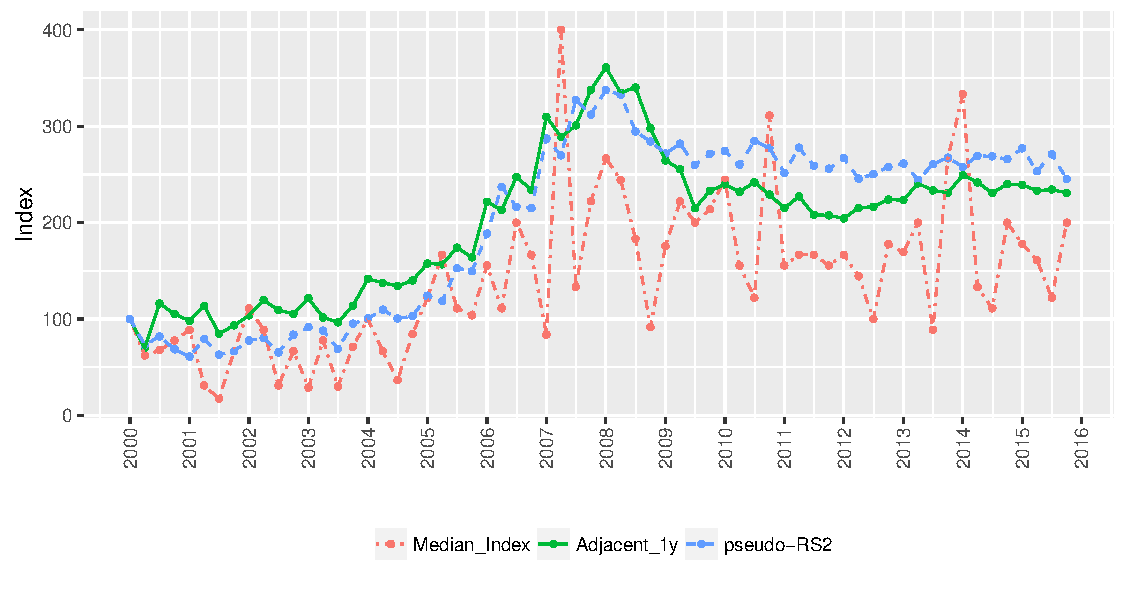
\includegraphics{Art_Price_Indices_5_J_files/figure-latex/figure10-1.pdf}
\caption{Comparing South African art price indices (2000Q1=100)}
\end{figure}

\begin{table}[ht]
\centering
\caption{Correlations in growth rates (dlogs)} 
\scalebox{0.9}{
\begin{tabular}{rllllllll}
  \hline
 & Median & Fisher & Hedonic & Adj1y & Adj2y & Roll & RepSale & ps.RS1 \\ 
  \hline
Median &  &  &  &  &  &  &  &  \\ 
  Fisher &  0.13  &  &  &  &  &  &  &  \\ 
  Hedonic &  0.03  &  0.38**  &  &  &  &  &  &  \\ 
  Adj1y &  0.09  &  0.32*  &  0.90*** &  &  &  &  &  \\ 
  Adj2y &  0.10  &  0.34**  &  0.95*** &  0.98*** &  &  &  &  \\ 
  Roll &  0.22  &  0.35**  &  0.94*** &  0.94*** &  0.95*** &  &  &  \\ 
  RepSale &  0.33*  &  0.00  & -0.12  & -0.08  & -0.03  & -0.09  &  &  \\ 
  ps.RS1 &  0.06  &  0.13  &  0.49*** &  0.60*** &  0.59*** &  0.51*** &  0.17  &  \\ 
  ps.RS2 &  0.05  &  0.13  &  0.49*** &  0.60*** &  0.60*** &  0.50*** &  0.34**  &  0.91*** \\ 
   \hline
\end{tabular}
}
\end{table}

All of the regression-based indices peak in 2008Q1, which is before the
peak in sales and annual median prices in the sample. All of the
measures indicate that quality-adjusted art prices increased
significantly between 2005 and 2008 and then declined relatively sharply
after the financial crisis, similar to other asset prices (Shimizu,
Nishimura, and Watanabe 2010). This conforms to the idea that there was
a surge in the popularity of South African art over the period, as well
as the idea of the formation of a bubble, with a dramatic rise and
subsequent decrease in prices.

The hedonic and ps-RS indices exhibit similar trends and high
correlations over the sample period, even though the hybrid repeat sales
indices are based on smaller subsamples of the data. This shows that
there is some consistency in the estimates from the different
methodologies. The ps-RS method provides a type of robustness check on
the hedonic indices. This provides some confidence that the indices
provide a relatively accurate measure of the price movements in the
South African art market and that the results are robust to changes in
methodology. It implies that the potential omitted variable and sample
selection bias may not be too pervasive in this case and are not driving
the dramatic price increases (Calomiris and Pritchett 2016).

\subsubsection{Evaluation}\label{evaluation}

This section evaluates the different art price indices in terms
smoothness, to determine which index provides the most credible gauge of
overall price movements in this case. In other applications, the quality
of price indices has often been evaluated based on the diagnostic
metrics of the underlying regressions, such as the standard errors of
the residuals (see e.g. Hansen (2009) for real estate indices).

However, Guo et al. (2014) argued that the regression residuals do not
represent errors in the price index, and hence do not directly reflect
inaccuracy in the index returns. Even if an index is perfectly accurate,
measuring the central tendency of market price changes in each period,
the regression would still have residuals and the time dummy
coefficients might still have large standard errors, resulting simply
from the dispersion of individual art prices around the central
tendency. When datasets become large, the regression diagnostics are
often good simply because of the size of the sample. In this case not
all of the indices are generated with regression models, and the
regressions models that are employed differ in their specifications (in
levels or first differences) and the underlying data used for
estimation.

Guo et al. (2014) suggested that signal-to-noise metrics, based directly
on the index produced, are a more appropriate for judging the quality of
the price index, as opposed to the underlying model. Random error in the
coefficient estimation leads to ``noise'' in the index. Signal-to-noise
metrics directly reflect the accuracy of the index returns and the
economic significance of random error in the indices. The volatility
(Vol) and the first order autocorrelations (AC(1)) of the index returns
are signal-to-noise metrics that may be useful to compare the amount of
noise in the indices.

The ideal price index filters out the noise-induced volatility to leave
only the true market volatility. In addition to the true volatility, the
noise (random error) in the index causes excess volatility in the index
returns. Excess volatility decreases the first order autocorrelation in
index returns. Other things being equal, the lower the volatility and
the higher the AC(1), the less noisy and more accurate the index. Thus,
lower Vol or higher AC(1) will indicate a better quality art price index
in the sense of less noise.

Guo et al. (2014) suggest another test of index quality in terms of
minimising random error that is based on the Hodrick-Prescott (HP)
filter. The HP filter is a spline fitting procedure that divides a time
series into smoothed trend and cyclical components. The idea is to
examine which index has the least deviation from its smoothed HP
component, by comparing the sum of squared differences between the index
returns and the smoothed returns.

Another option is to compare the smoothness coefficients proposed by
Froeb and Koyak (1994). The smoothness coefficient is defined as the
average long run variance of a time series divided by the average short
run variance. The idea is to obtain the spectral density of the time
series, which shows the contribution of all frequencies to the data
series. The smoothness measure is then taken as the average of the lower
half of the frequency range (i.e.~low frequency movements) over the
average of the upper half of the frequencies (i.e.~higher frequencies).
A higher smoothness coefficient indicates a larger portion of variance
in the low frequencies and a smoother time series.

Table 2 reports these four metrics of index smoothness for the art price
indices. The 1-year adjacent period hedonic index performs the best in
terms of these metrics, with the lowest volatility and highest AC(1) in
returns, the smallest deviation from its smoothed returns, and the
highest smoothness coefficient. However, the smoothness coefficients of
the regression-based indices are not significantly different.

\begin{table}[ht]
\centering
\caption{Smoothness Indicators} 
\scalebox{0.9}{
\begin{tabular}{rrrrr}
  \hline
 & Vol & AC.1 & HPDeviation & Smoothness \\ 
  \hline
Median & 0.612 & -0.416 & 22.11 & -0.02 \\ 
  Fisher & 0.284 & -0.332 & 4.66 & 1.00 \\ 
  Hedonic & 0.114 & -0.323 & 0.75 & 1.09 \\ 
  Adj1y & 0.105 & -0.246 & 0.63 & 1.39 \\ 
  Adj2y & 0.105 & -0.303 & 0.63 & 1.10 \\ 
  Roll & 0.112 & -0.279 & 0.73 & 1.27 \\ 
  RepSale & 0.549 & -0.403 & 17.76 & 0.65 \\ 
  ps.RS1 & 0.128 & -0.360 & 0.95 & 0.94 \\ 
  ps.RS2 & 0.123 & -0.342 & 0.87 & 1.16 \\ 
   \hline
\end{tabular}
}
\end{table}

\subsection{Bubble Detection Results}\label{bubble-detection-results}

This section tests whether the South African art market has exhibited
bubble-like behaviour over the sample period, focusing on a specific
aspect of bubbles: explosive prices. This section follows the convention
of using the log value of real asset prices, deflated with the CPI (e.g.
Kräussl, Lehnert, and Martelin (2016), Caspi (2013) and Balcilar,
Katzke, and Gupta (2015)). In this case there is only one potential
bubble episode, so the Peter C B Phillips, Wu, and Yu (2011) method
should be sufficient to provide consistent evidence of mildly explosive
behaviour.

The model starts with 3 years and expands the sample by one observation
each time. In this case, there does not seem to be a deterministic drift
present in the log real art price indices and the intercept is not
statistically significant at conventional levels. In their original
study Peter C B Phillips, Wu, and Yu (2011) use a random walk without
drift to estimate the null hypothesis. Peter C B Phillips, Shi, and Yu
(2014) argue that an empirically more realistic description of explosive
behaviour is given by models formulated without a drift or deterministic
trend. Nevertheless, as a robustness check the models were formulated
with and without a drift term included. Lags are included to take
possible autocorrelation of the residuals into account and the number of
lags \(k\) is chosen with the Akaike Information Criterion. Critical
values for the tests are derived from Monte Carlo simulations of a
random walk process, both including and excluding a drift term, with
2000 replications.

The supremum ADF test statistics from to both formulations are above the
95\% critical values for each of the indices, except for the median
index. Therefore, the null hypothesis of a unit root may be rejected in
favour of the alternative hypothesis for each of the indices, except the
median index. Figure 2 illustrates the date stamping procedure for three
representative series (without drift): the median index, the 1-year
adjacent period hedonic index and the second version (larger sample) of
the ps-RS index. The figures compare the ADF test static sequence to the
95\% and 99\% critical value sequences. In both cases the test statistic
sequences breach the 95\% critical values in the run-up to the financial
crisis (2005 and 2006 respectively), before falling below the critical
values. The sequence of test statistics for the ps-RS index is higher
than for the hedonic index, and breaches the 99\% critical value.

\begin{figure}[htbp]
\centering
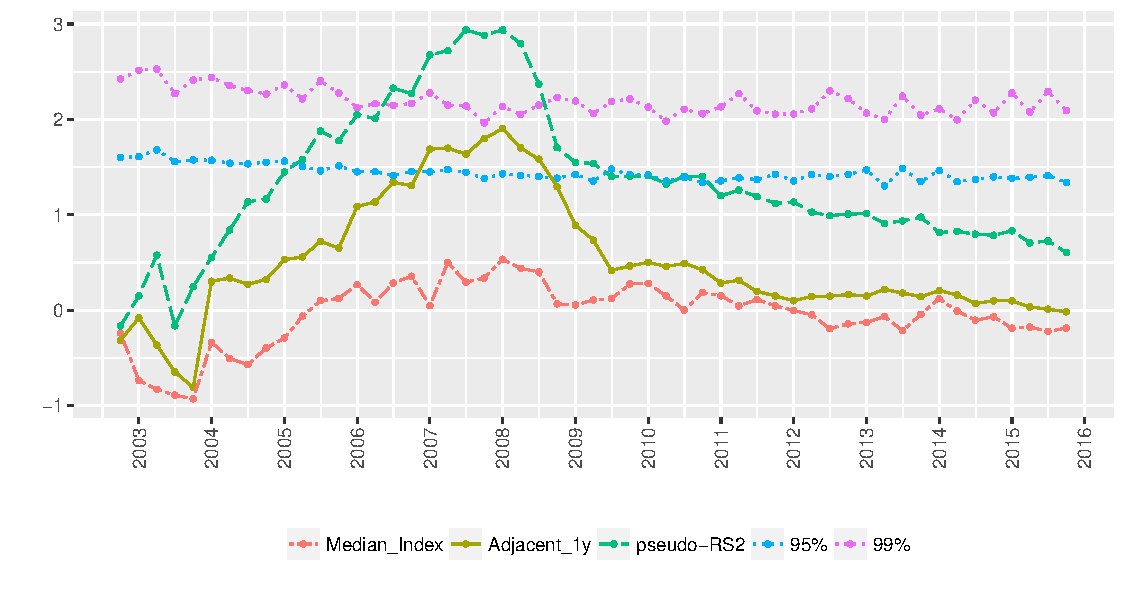
\includegraphics{Art_Price_Indices_5_J_files/figure-latex/figure15-1.pdf}
\caption{Test statistics and critical values for models without drift}
\end{figure}

Table 3 reports the origination and termination dates for all of the
indices, based on 95\% critical values. The test statistic sequences for
the hedonic indices all indicate a period of explosive prices beginning
around 2006/2007 and ending in 2008. The test statistics for the ps-RS
indices indicate periods of explosive behaviour that were slightly
longer, beginning around 2005/2006 and ending in 2008 or even 2010,
depending on the specification. The preferred index in terms of
smoothness (i.e.~the 1-year adjacent index) suggests a period of bubble
formation from 2007Q1 to 2008Q3. Peter Charles Bonant Phillips, Shi, and
Yu (2012) recommend that only explosive periods lasting more than log(T)
units of time should be identified as bubble periods. In this case this
implies that the bubble should be at least 4 quarters in length and
virtually all of the explosive periods identified satisfy this
requirement.

\begin{table}[ht]
\centering
\caption{Dates of explosive behaviour} 
\scalebox{0.9}{
\begin{tabular}{rllll}
  \hline
  & \multicolumn{2}{c}{  No Drift  } & \multicolumn{2}{c}{ Drift }\\ \hline
  & Start & End & Start & End \\ 
  Fisher\_Index & 2008 Q1 & 2010 Q3 & 2008 Q1 & 2009 Q2 \\ 
  Hedonic\_full & 2007 Q1 & 2008 Q3 & 2007 Q1 & 2008 Q2 \\ 
  Adjacent\_1y & 2007 Q1 & 2008 Q3 & 2006 Q3 & 2008 Q2 \\ 
  Adjacent\_2y & 2007 Q1 & 2008 Q4 & 2006 Q3 & 2008 Q2 \\ 
  Rolling\_5y & 2007 Q2 & 2008 Q3 & 2007 Q1 & 2008 Q2 \\ 
  pseudo-RS1 & 2006 Q1 & 2010 Q1 & 2006 Q1 & 2008 Q2 \\ 
  pseudo-RS2 & 2005 Q2 & 2010 Q4 & 2004 Q2 & 2008 Q2 \\ 
   \hline
\end{tabular}
}
\end{table}

The dates identified correspond with many of the explosive periods
identified in the literature for a range of assets. In the context of
art, Kräussl, Lehnert, and Martelin (2016) identified bubble periods for
the ``\emph{Post-war and Contemporary}'' art segment between 2006 and
2008 and for the ``\emph{American}'' art segments between 2005 and 2008,
which also corresponds to the pre-financial crisis period. They found
evidence of the formation of another bubble in these market segments
around the start of 2011. This is not present in the South African art
market, which has remained relatively flat since 2010. This is mirrored
by South Africa's experience during the Great Recession, which was not
as deep as in most developed countries, but was more protracted.

\subsubsection{Art Market Segments}\label{art-market-segments}

Different segments of the South African art market exhibit different
price trends over time. This section examines different segments of the
market, in order to establish in which segments the marked price
increases occurred. The caveat is that slicing the data thinly results
in small sample sizes and more volatile indices. This makes it more
difficult to discern a pattern and to distinguish the signal from the
noise.

The South African art market may be segmented for a number of reasons.
Small investors are generally not able to invest in more expensive
works, while wealthy individuals may be less tempted to buy at the lower
end of the market, where works do not signal the same social status. The
more expensive parts of the market may be more prone to speculation
(Renneboog and Spaenjers 2013). Fedderke and Li (2014) suggested that
the South African art market should be segmented into three price ranges
and found different hedonic relationships for the three market segments.

Thus, historical rates of appreciation may have varied across the price
distribution (Renneboog and Spaenjers 2013). In order to test this
possibility, different part of the price distribution may be
investigated separately by estimating hedonic indices for different
parts of the distribution. Three indices are estimated for the bottom
25\% of the price distribution (``Lower''), the interquartile range
(``Middle''), and the upper 25\% of the distribution
(``Upper'').\footnote{The models are estimated with the full sample
  hedonic method. The models include dummy variables for all the artists
  that sold more than one artwork during the sample period. The
  adjacent-period hedonic and ps-RS models are used to confirm the
  results. In many cases, however, there are too few observations to
  estimate full indices.} The indices suggest that the dramatic price
increases occurred in the upper part of the price distribution, which
includes artworks with a hammer price of more than R22,000.

The market may also be segmented by artist value. In order to examine
the price appreciation of the more expensive artists' work, the artists
are ranked according to the average value of their artworks sold in the
sample (i.e.~average price per artwork). Separate hedonic regression
were estimated for the bottom 25\% of the value distribution (i.e.~for
all artists in the lower part of the value distribution), the
interquartile range, and the upper 25\% of the distribution. Price
increased more dramatically for artworks by the more expensive artists,
which in this case includes the top 262 artists in terms of average
price per artwork.

Another potential segmentation is by medium category. It is possible
that historical rates of appreciation have varied widely over time for
specific media. Separate hedonic models may be estimated for each of the
different mediums. Oil paintings are by far the largest category,
representing 52\% of the volume and 78\% of the value of artworks in the
sample. The indices indicate that oil was the medium that experienced
the largest price increases.

Finally, quantile regressions provide an alternative means to
investigate different parts of the price distribution and are also more
robust to potential outliers. OLS regressions provide estimates for the
conditional means, whereas quantile regressions can characterise the
entire distribution of the dependent variable. The indices resulting
from quantile regressions for the 25th, 50th, and 75th percentiles are
relatively similar. The lower end of the market seems to have
depreciated slightly less after the peak in 2008. Overall the results
seem to indicate that the dramatic price increases occurred in more
expensive or high-end parts of the art market, and especially for oil
paintings.

The results for the origination and termination dates are reported in
Table 4. The results indicate that the bubble process was relatively
dispersed throughout the market. Although prices seem to have been
especially explosive for high-end oil paintings by top artists, the
bubble detection tests also provide some evidence of explosive prices
for other medium categories and less expensive artists. The origination
and termination dates also seem to be relatively consistent in
suggesting a bubble formation period between 2006/07 and 2008.

\begin{table}[ht]
\centering
\caption{Dates of explosive behaviour by segment} 
\scalebox{0.9}{
\begin{tabular}{rllll}
  \hline
  & \multicolumn{2}{c}{  No Drift  } & \multicolumn{2}{c}{ Drift }\\ \hline
  & Start & End & Start & End \\ 
  price\_lower &  &  &  &  \\ 
  price\_middle &  &  &  &  \\ 
  price\_upper &  &  & 2007 Q1 & 2008 Q1 \\ 
  value\_lower & 2002 Q4 & 2010 Q1 & 2007 Q4 & 2009 Q2 \\ 
  value\_middle & 2006 Q3 & 2008 Q4 & 2006 Q1 & 2008 Q4 \\ 
  value\_upper & 2007 Q4 & 2008 Q1 & 2007 Q2 & 2008 Q1 \\ 
  Drawing &  &  &  &  \\ 
  Watercolour & 2007 Q3 & 2008 Q2 & 2007 Q3 & 2008 Q1 \\ 
  Oil & 2006 Q2 & 2009 Q2 & 2006 Q2 & 2008 Q2 \\ 
  Print/Woodcut & 2007 Q4 & 2008 Q3 &  &  \\ 
  Mixed Media & 2007 Q1 & 2009 Q2 &  &  \\ 
  Sculpture &  &  & 2007 Q2 & 2007 Q3 \\ 
  tau=0.25 &  &  &  &  \\ 
  tau=0.50 &  &  &  &  \\ 
  tau=0.75 &  &  & 2007 Q2 & 2008 Q1 \\ 
   \hline
\end{tabular}
}
\end{table}

\section{Discussion}\label{discussion}

The regression-based indices provide relatively consistent results in
terms of the explosive periods in the South African art market, with a
potential bubble most likely beginning in 2006 and ending in 2008.
Although the method provides a consistent basis for identifying periods
of explosive behaviour, it does not provide an explanation of the bubble
episode. The findings are compatible with several different
explanations, including rational bubbles, herd behaviour, and rational
responses to fundamentals (Peter C B Phillips, Wu, and Yu 2011).

The results implicitly assume that the aesthetic or utility dividends
associated with South African art did not exhibit explosive behaviour
over the period. Aesthetic dividends fluctuate over time as they depend
on buyers' willingness to pay for art, which in turn depends on
preferences and wealth. However, preferences regarding art and culture
would have had to fluctuate dramatically to explain the movements in art
prices over the period. Even if trends can temporarily emerge for
specific artists or schools of art, previous findings in the literature
have shown that preferences tend to be very stable, even in the long run
(Penasse and Renneboog 2014). The aesthetic dividend can also fluctuate
as wealth fluctuates over time (Spaenjers, Goetzmann, and Mamonova
2015). The literature has provided evidence supporting this idea, with
W. Goetzmann, Renneboog, and Spaenjers (2011) finding cointegrating
relationships between top incomes and art prices. However, it is
unlikely that aesthetic dividends, or factors such as collectors'
preferences and wealth, experienced similar explosive behaviour over the
period.

The large increase in art prices between 2005 and 2008 does not seem to
be due to a fundamental shift in the types of artworks that were sold
over that period. For instance, the top 100 artists in terms of volumes
sold, which accounts for 60\% of the volume traded and 90\% of total
turnover, has remained remarkably stable over time. Even if the exact
same artworks were not being resold, the same artists' work still made
up the vast majority of the market, and the hedonic model controls for
the different artists. It is unlikely that the results are driven by
sales of systematically better or higher quality artworks by specific
artists that appreciated in price over that period, and by sales of
systematically lower quality artworks by those artists after the crisis.
Moreover, paintings are not sold at auction only to profit from price
appreciation or capital gains. A substantial portion of consignments
come from the so-called three D's: Debt, Divorce and Death. In other
words, many sellers are forced to sell their artworks, even if those
artworks have not experienced the largest price appreciation.

Penasse and Renneboog (2014) argue that limits to arbitrage induce a
speculative component to art prices. High transaction costs and
short-selling constraints could lead to prices diverging from
fundamental levels, as they prevent arbitrageurs from pulling back
prices to fundamentals (Balcilar, Katzke, and Gupta 2015). When prices
are high, pessimists would like to short sell, but instead simply stay
out of the market or sell to optimists at inflated prices. Optimists may
be willing to pay higher prices than their own valuations, because they
expect to resell to even more optimistic investors in the future. The
difference between their willingness to pay and their own optimistic
valuation is the price of the option to resell the asset in the future.
The price of the resale option imparts a bubble component in asset
prices, and can explain price fluctuations unrelated to fundamentals.
These market failures hamper the ability of markets to correct price
inefficiencies and implies that periods of bubble-like behaviour could
exist with relatively little scope for arbitrage. This is especially
applicable to art markets, where transaction costs are high, short
selling is not possible, and without a rental market the only
possibility to make a profit is by reselling at a higher price (Penasse
and Renneboog 2014).

Kindleberger and Aliber (2005) argued that a boom in one market often
spills over into other markets. A famous example in the context of art
is the link between the boom in Japanese stock and real estate prices
and the Impressionist art market in the second half of the 1980s. Hiraki
et al. (2009) found a strong correlation between Japanese stock prices
and the demand for art by Japanese collectors, leading to an increase in
the price of Impressionist art during this period. Kräussl, Lehnert, and
Martelin (2016) found corroborating evidence of a bubble period in the
``Impressionist and Modern'' art segment between 1986 and 1991. During
this period Japanese credit was freely available, backed by increasing
values of stocks and real estate, which led to a consumption and
investment spree through the wealth effect. Japanese investors invested
heavily in international art and particularly French Impressionist art
in the late 1980s. Luxury consumption by Japanese art collectors
increased international art prices until the art bubble burst as a
direct consequence of the collapse of the Japanese real estate market
(Penasse and Renneboog 2014).

Similarly, the run-up to the financial crisis saw large increases in
asset prices and credit expansion in South Africa. It is likely that
these conditions contributed to the explosive behaviour in South African
art prices between 2006 and 2008. The financial crisis caused the bubble
to burst and led to a decline in South African art prices.

\section{Conclusion}\label{conclusion}

This paper used a direct method of bubble detection developed by Peter C
B Phillips, Wu, and Yu (2011) to test for explosive behaviour in South
African art prices. The test requires the estimation of a reasonably
accurate quality-adjusted price index, which can be challenging for
unique assets such as art. Each methodology has shortcomings and the
danger is that the biases inherent in each methodology may be driving
the results. This paper estimates three sets of art price indices, based
on the three main methodologies used to estimate quality-adjusted price
indices for unique assets.

The regression-based indices seem to point to consistent evidence of
mildly explosive price behaviour in the run-up to the financial crisis,
between 2005/06 and 2008. The bubble seems to have been relatively
dispersed throughout the market, although prices seem to have been
especially explosive for high-end oil paintings by the top artists.

\section*{References}\label{references}
\addcontentsline{toc}{section}{References}

\hypertarget{refs}{}
\hypertarget{ref-Anderson1974}{}
Anderson, R. C. 1974. ``Paintings as an investment.'' \emph{Economic
Inquiry} 12: 13--26.

\hypertarget{ref-Areal2013}{}
Areal, Francisco J, Kelvin Balcombe, and George Rapsomanikis. 2013.
``Testing for bubbles in agriculture commodity markets.'' \emph{Munich
Personal RePEc Archive}, MPRA paper no. 48015, no. 48015.

\hypertarget{ref-Bailey1963a}{}
Bailey, Martin J, Richard F Muth, and Hugh O Nourse. 1963. ``A
regression method for real estate price index construction.''
\emph{Journal of the American Statistical Association} 58 (304):
933--42.
doi:\href{https://doi.org/10.1080/01621459.1963.10480679}{10.1080/01621459.1963.10480679}.

\hypertarget{ref-Balcilar2015}{}
Balcilar, Mehmet, Nico Katzke, and Rangan Gupta. 2015. ``Identifying
Periods of US Housing Market Explosivity.'' \emph{University of
Pretoria: Department of Economics Working Paper Series} 2015-44.

\hypertarget{ref-Brunnermeier2008}{}
Brunnermeier, Markus K. 2008. ``Bubbles.'' In \emph{New Palgrave
Dictionary of Economics}, edited by Steven N. Durlauf and Lawrence E.
Blume, 2nd ed., 1--17. i. Palgrave Macmillan.

\hypertarget{ref-Calomiris2016}{}
Calomiris, By Charles W, and Jonathan Pritchett. 2016. ``Betting on
Secession: Quantifying Political Events Surrounding Slavery and the
Civil War.'' \emph{American Economic Review} 106 (1): 1--23.

\hypertarget{ref-Campbell1987}{}
Campbell, John Y., and Robert J Shiller. 1987. ``Cointegration and Tests
of Present Value Models.'' \emph{The Journal of Political Economy} 95
(5): 1062--88.
doi:\href{https://doi.org/10.1086/261502}{10.1086/261502}.

\hypertarget{ref-Candela2001}{}
Candela, Guido, and Antonello Eugenio Scorcu. 2001. ``In search of
stylized facts on art market prices: Evidence from the secondary market
for prints and drawings in Italy.'' \emph{Journal of Cultural Economics}
25 (3): 219--31.
\url{http://www.springerlink.com/index/P15X134NX82538R1.pdf}.

\hypertarget{ref-Case1987}{}
Case, Karl E, and Robert J Shiller. 1987. ``Prices of single-family
homes since 1970: new indexes for four cities.'' \emph{New England
Economic Review}, no. September: 45--56.
doi:\href{https://doi.org/10.3386/w2393}{10.3386/w2393}.

\hypertarget{ref-Caspi2013}{}
Caspi, Itamar. 2013. ``Rtadf: Testing for Bubbles with EViews.''
\emph{Munich Personal RePEc Archive}, no. 58791.

\hypertarget{ref-Curnow2010}{}
Curnow, Robyn. 2010. ``South Africa's Booming Art Market.'' \emph{CNN
World}.
\url{http://edition.cnn.com/2010/WORLD/africa/06/17/kentridge.south.africa.art.star/}.

\hypertarget{ref-Deng2012}{}
Deng, Y, D McMillen, and T Sing. 2012. ``Private Residential Price
Indices in Singapore: A Matching Approach.'' \emph{Regional Science and
Urban Economics} 42 (3): 485--94.

\hypertarget{ref-Diba1988}{}
Diba, Behzad T., and Herschel I. Grossman. 1988. ``The Theory of
Rational Bubbles in Stock Prices.'' \emph{Economic Journal} 98 (392):
746--54.

\hypertarget{ref-Dorsey2010}{}
Dorsey, Robert E., Haixin Hu, Walter J. Mayer, and Hui Chen Wang. 2010.
``Hedonic versus repeat-sales housing price indexes for measuring the
recent boom-bust cycle.'' \emph{Journal of Housing Economics} 19 (2).
Elsevier Inc.: 87--105.
doi:\href{https://doi.org/10.1016/j.jhe.2010.04.001}{10.1016/j.jhe.2010.04.001}.

\hypertarget{ref-Eurostat2013}{}
Eurostat. 2013. \emph{Handbook on Residential Property Price Indices
(RPPIs)}. November 2009. Luxembourg: Publications Office of the European
Union, 2013: European Commission.

\hypertarget{ref-Evans1991}{}
Evans, G W. 1991. ``Pitfalls in Testing for Explosive Bubbles in Asset
Prices.'' \emph{American Economic Review} 81 (4): 922--30.
doi:\href{https://doi.org/10.2307/2006651}{10.2307/2006651}.

\hypertarget{ref-Fedderke2014}{}
Fedderke, Johannes W, and Kaini Li. 2014. ``Art in Africa: Market
Structure and Pricing Behavior in the South African Fine Art Auction
Market, 2009-2013.'' Economic Research Southern Africa.

\hypertarget{ref-Figuerola2015}{}
Figuerola-Ferretti, Isabel, Christopher L Gilbert, and Roderick
Mccrorie. 2015. ``Testing for Bubbles in LME Non-Ferrous Metals
Prices.'' \emph{Journal of Time Series Analysis} 36: 763--82.

\hypertarget{ref-Froeb1994}{}
Froeb, Luke, and Robert Koyak. 1994. ``Measuring and Comparing
Smoothness in Time Series: The Production Smoothing Hypothesis.''
\emph{Journal of Econometrics} 64: 97--122.

\hypertarget{ref-Gerard-Varet1995}{}
Gérard-Varet, L. V. 1995. ``On pricing the priceless: Comments on the
economics of the visual art market.'' \emph{European Economic Review}
39: 509--18.

\hypertarget{ref-Goetzmann2011}{}
Goetzmann, William, Luc Renneboog, and Christophe Spaenjers. 2011. ``Art
And Money.'' \emph{The American Economic Review} 101 (3): 222--46.

\hypertarget{ref-Griliches1961}{}
Griliches, Zvi. 1961. \emph{Hedonic Price Indexes for Automobiles: An
Econometric of Quality Change}. National Bureau of Economic Research.
doi:\href{https://doi.org/10.1017/CBO9781107415324.004}{10.1017/CBO9781107415324.004}.

\hypertarget{ref-Guo2014}{}
Guo, Xiaoyang, Siqi Zheng, David Geltner, and Hongyu Liu. 2014. ``A new
approach for constructing home price indices: The pseudo repeat sales
model and its application in China.'' \emph{Journal of Housing
Economics} 25. Elsevier Inc.: 20--38.
doi:\href{https://doi.org/10.1016/j.jhe.2014.01.005}{10.1016/j.jhe.2014.01.005}.

\hypertarget{ref-Hansen2009}{}
Hansen, James. 2009. ``Australian house prices: A comparison of hedonic
and repeat-sales measures.'' \emph{Economic Record} 85: 132--45.
doi:\href{https://doi.org/10.1111/j.1475-4932.2009.00544.x}{10.1111/j.1475-4932.2009.00544.x}.

\hypertarget{ref-Hiraki2009}{}
Hiraki, Takato, Akitoshi Ito, Darius a. Spieth, and Naoya Takezawa.
2009. ``How Did Japanese Investments Influence International Art
Prices?'' \emph{Journal of Financial and Quantitative Analysis} 44 (06):
1489.
doi:\href{https://doi.org/10.1017/S0022109009990366}{10.1017/S0022109009990366}.

\hypertarget{ref-Homm2012}{}
Homm, Jörg, and Ulrich Breitung. 2012. ``Testing for Speculative Bubbles
in Stock Markets: A Comparison of Alternative Methods.'' \emph{Journal
of Financial Econometrics} 12 (1): 198--231.

\hypertarget{ref-Hundt2010}{}
Hundt, Stefan. 2010. ``Art Auction Round-Up.'' \emph{SANLAM Private
Investments Art Advisory Service}.

\hypertarget{ref-Jiang2014}{}
Jiang, Liang, Peter C B Phillips, and Jun Yu. 2014. ``A New Hedonic
Regression for Real Estate Prices Applied to the Singapore Residential
Market.'' \emph{Cowles Foundation Discussion Paper No. 1969}.

\hypertarget{ref-Kindleberger2005}{}
Kindleberger, Charles P, and Robert Z Aliber. 2005. \emph{Manias,
Panics, and Crashes}. 5th ed. Hoboken, New Jersey: John Wiley \& Sons,
Inc.

\hypertarget{ref-Korteweg2013}{}
Korteweg, Arthur G. 2013. ``Research: Is Art A Good Investment?''
\emph{Stanford Business}.

\hypertarget{ref-Kraussl2014}{}
Kräussl, Roman. 2015. ``Art as an alternative asset class: Risk and
return characteristics of the Middle Eastern \& Northern African art
markets.'' In \emph{Cosmopolitan Canvases}, edited by Olav Velthuis and
Stefano Baia Curioni. Oxford University Press: Oxford.
doi:\href{https://doi.org/10.1093/acprof:oso/9780198717744.001.0001}{10.1093/acprof:oso/9780198717744.001.0001}.

\hypertarget{ref-Kraussl2010}{}
Kräussl, Roman, and Jonathan Lee. 2010. ``Art as an Investment: the Top
500 Artists.'' \emph{Business} 31 (February): 1--26.

\hypertarget{ref-Kraussl2010a}{}
Kräussl, Roman, and Robin Logher. 2010. ``Emerging art markets.''
\emph{Emerging Markets Review} 11: 301--18.
doi:\href{https://doi.org/10.1016/j.ememar.2010.07.002}{10.1016/j.ememar.2010.07.002}.

\hypertarget{ref-Kraussl2008}{}
Kräussl, Roman, and Niels Van Elsland. 2008. ``Constructing the true art
market index: a novel 2-step hedonic approach and its application to the
german art market.'' \emph{Center for Financial Studies} 2008/11.

\hypertarget{ref-Kraussl2016}{}
Kräussl, Roman, Thorsten Lehnert, and Nicolas Martelin. 2016. ``Is there
a bubble in the art market?'' \emph{Journal of Empirical Finance} 35.
Elsevier B.V.: 99--109.
doi:\href{https://doi.org/10.1016/j.jempfin.2015.10.010}{10.1016/j.jempfin.2015.10.010}.

\hypertarget{ref-Lancaster1966}{}
Lancaster, Kelvin J. 1966. ``A New Approach to Consumer Theory.''
\emph{The Journal of Political Economy} 74 (2): 132--57.

\hypertarget{ref-Mandel2009}{}
Mandel, Benjamin R. 2009. ``Art as an Investment and Conspicuous
Consumption Good.'' \emph{The American Economic Review} 99 (4):
1653--63.
doi:\href{https://doi.org/10.1257/aer.99.4.1653}{10.1257/aer.99.4.1653}.

\hypertarget{ref-McMillen2012}{}
McMillen, Daniel P. 2012. ``Repeat Sales as a Matching Estimator.''
\emph{Real Estate Economics} 40 (4): 743--71.
doi:\href{https://doi.org/10.1111/j.1540-6229.2012.00343.x}{10.1111/j.1540-6229.2012.00343.x}.

\hypertarget{ref-Mei2002}{}
Mei, Jianping, and Michael Moses. 2002. ``Art as an investment and the
underperformance of masterpieces.'' \emph{American Economic Review} 92
(February): 1656--68.
doi:\href{https://doi.org/10.1257/000282802762024719}{10.1257/000282802762024719}.

\hypertarget{ref-Naidoo2013}{}
Naidoo, Prakash. 2013. ``Art Market: Auction houses reflect SA.''
\url{http://www.financialmail.co.za/life/2013/08/22/art-market-auction-houses-reflect-sa}.

\hypertarget{ref-Olckers2015}{}
Olckers, Matthew, Catherine Kannemeyer, and Michael Stevenson. 2015.
``Art Critic Index : A Proxy for Cultural Value in the Context of the
South Africa Art Market.'' \emph{ERSA Working Paper}, ERSA working
paper, 500 (February). Economic Research Southern Africa.

\hypertarget{ref-Penasse2014}{}
Penasse, Julien, and Luc Renneboog. 2014. ``Bubbles and Trading
Frenzies: Evidence from the Art Market.'' \emph{CentER Discussion Paper}
2014-068. CentER Discussion Paper.

\hypertarget{ref-Phillips2014}{}
Phillips, Peter C B, Shuping Shi, and Jun Yu. 2014. ``Specification
Sensitivity in Right-Tailed Unit Root Testing for Explosive Behaviour.''
\emph{Oxford Bulletin of Economics and Statistics} 76 (3): 315--33.
doi:\href{https://doi.org/10.1111/obes.12026}{10.1111/obes.12026}.

\hypertarget{ref-Phillips2011}{}
Phillips, Peter C B, Yangru Wu, and Jun Yu. 2011. ``Explosive Behavior
In The 1990S Nasdaq: When Did Exuberance Escalate Asset Values?''
\emph{International Economic Review} 52 (1): 201--26.
doi:\href{https://doi.org/10.1111/j.1468-2354.2010.00625.x}{10.1111/j.1468-2354.2010.00625.x}.

\hypertarget{ref-Phillips2012}{}
Phillips, Peter Charles Bonant, Shu-Ping Shi, and Jun Yu. 2012.
``Testing for Multiple Bubbles.'' \emph{Cowles Foundation for Research
in Economics}, no. 1843.

\hypertarget{ref-Rabe2011}{}
Rabe, Jo-Marie. 2011. ``Beautiful bubbles burst.'' \emph{Personal
Finance Magazine}, October.

\hypertarget{ref-Renneboog2012}{}
Renneboog, Luc, and Christophe Spaenjers. 2013. ``Buying Beauty: On
Prices and Returns in the Art Market.'' \emph{Management Science} 59
(1): 36--53.
doi:\href{https://doi.org/10.1287/mnsc.1120.1580}{10.1287/mnsc.1120.1580}.

\hypertarget{ref-Renneboog2014}{}
---------. 2015. ``Investment Returns and Economic Fundamentals in
International Art Markets.'' In \emph{Cosmopolitan Canvases}, edited by
Olav Velthuis and Stefano Baia Curioni. Oxford University Press: Oxford.
doi:\href{https://doi.org/10.1093/acprof:oso/9780198717744.001.0001}{10.1093/acprof:oso/9780198717744.001.0001}.

\hypertarget{ref-Renneboog2002}{}
Renneboog, Luc, and Tom Van Houtte. 2002. ``The monetary appreciation of
paintings: from realism to Magritte.'' \emph{Cambridge Journal of
Economics} 26: 331--57.
doi:\href{https://doi.org/10.1093/cje/26.3.331}{10.1093/cje/26.3.331}.

\hypertarget{ref-Rosen1974}{}
Rosen, Sherwin. 1974. ``Hedonic Prices and Implicit Markets : Product
Differentiation in Pure Competition Authors.'' \emph{Journal of
Political Economy} 82 (1): 34--55.

\hypertarget{ref-Shimizu2010}{}
Shimizu, Chihiro, Kiyohiko G. Nishimura, and Tsutomu Watanabe. 2010.
``Housing Prices in Tokyo: A comparison of hedonic and repeat sales
measures.'' \emph{Jahrbucher Fur Nationalokonomie Und Statistik} 230
(6): 792--813.

\hypertarget{ref-Spaenjers2015}{}
Spaenjers, Christophe, William N. Goetzmann, and Elena Mamonova. 2015.
``The economics of aesthetics and record prices for art since 1701.''
\emph{Explorations in Economic History} 57. Elsevier Inc.: 79--94.
doi:\href{https://doi.org/10.1016/j.eeh.2015.03.003}{10.1016/j.eeh.2015.03.003}.

\hypertarget{ref-Triplett2004}{}
Triplett, Jack. 2004. ``Handbook on Hedonic Indexes and Quality
Adjustments in Price Indexes: Special Application To Information
Technology Products.'' OECD.
doi:\href{https://doi.org/10.1787/643587187107}{10.1787/643587187107}.

\hypertarget{ref-Yiu2013}{}
Yiu, Matthew S., Jun Yu, and Lu Jin. 2013. ``Detecting Bubbles in Hong
Kong Residential Property Market.'' \emph{Journal of Asian Economics} 28
(October): 115--24.

\end{document}


